\documentclass{beamer}
\usepackage{beamerthemesplit}
\usepackage{wrapfig}
\usetheme{SPbGU}
\usepackage{pdfpages}
\usepackage{amsmath}
\usepackage{mathtools}
\usepackage{cmap} 
\usepackage[T2A]{fontenc} 
\usepackage[utf8]{inputenc}
\usepackage[english,russian]{babel}
\usepackage{indentfirst}
\usepackage{amsmath}
\usepackage{tikz}
\usepackage{multirow}
\usepackage[noend]{algpseudocode}
\usepackage{algorithm}
\usepackage{algorithmicx}
\usepackage{ stmaryrd }
\usepackage{qtree}
\usetikzlibrary{shapes,arrows}
\usepackage{fancyvrb}
\usepackage{minted}
\newtheorem{rutheorem}{Теорема}
\newtheorem{ruproof}{Доказательство}
\newtheorem{rudefinition}{Определение}
\newtheorem{rulemma}{Лемма}
\beamertemplatenavigationsymbolsempty

\newcommand{\derive}[0]{\xRightarrow[]{*}}
\newcommand{\derives}[0]{\xRightarrow[]{}}
\newcommand{\derivek}[1]{\xRightarrow[]{#1}}
\newcommand{\deriveg}[1]{\xRightarrow[#1]{*}}
\newcommand{\derivegone}[1]{\xRightarrow[#1]{}}

\title[]{Теория автоматов и формальных языков}
\subtitle[]{Parsing expression grammar}
\institute[]{
Санкт-Петербургский государственный электротехнический университет <<ЛЭТИ>>\\
}

\author[]{Екатерина Вербицкая}

\date{1 ноября 2016г.}

\definecolor{orange}{RGB}{179,36,31}

\begin{document}
{
  \begin{frame}
    \titlepage
  \end{frame}
}

\begin{frame}[fragile]
  \transwipe[direction=90]
  \frametitle{В предыдущей серии}
  \begin{itemize}
    \item Нисходящий анализ
    \item Множество $FIRST$
    \item Множество $FOLLOW$
    \item Удаление левой рекурсии
    \item Факторизация грамматики
    \item $LL(1)$-таблица
    \item $LL(1)$ синтаксический анализ
  \end{itemize}
\end{frame}

\begin{frame}[fragile]
  \transwipe[direction=90]
  \frametitle{В предыдущей серии}
  \begin{itemize}
	\item Преимущества $LL(1)$ синтаксического анализа
	\begin{itemize}
	  \item Прост и понятен
	  \item Разбор за $O(n)$, где $n$ --- длина входной строки
	  \item Применим для многих практически полезных задач (с оговорками)
	\end{itemize}
    \item Недостатки $LL(1)$ синтаксического анализа
    \begin{itemize}
      \item Необходимость преобразовывать грамматику
      \item Достаточно небольшой класс языков, которые действительно можно разобрать синтаксическим анализатором
    \end{itemize}
  \end{itemize}
\end{frame}

\begin{frame}[fragile]
  \transwipe[direction=90]
  \frametitle{Dangling else problem}
  \begin{itemize}
    \item Грамматика для условного оператора $if$
    \begin{itemize}
      \item $E \rightarrow b $
      \item $S \rightarrow \underline{if} \, E \, \underline{then} \, S \, \underline{else} \, S \, | \, \underline{if} \, E \, \underline{then} \, S \, | \, a$    
    \end{itemize}
    
    \item $\underline{if} \, b \, \underline{then} \, a  \, \underline{if} \, b \, \underline{then} \, a \, \underline{else} \, a$ \pause
    \begin{itemize}
      \item $\underline{if} \, b \, \underline{then} \, a  \, (\underline{if} \, b \, \underline{then} \, a \, \underline{else} \, a)$
      \item $\underline{if} \, b \, \underline{then} \, a  \, (\underline{if} \, b \, \underline{then} \, a) \, \underline{else} \, a$
    \end{itemize}
  \end{itemize}
\end{frame}

\begin{frame}[fragile]
  \transwipe[direction=90]
  \frametitle{Dangling else problem}
  \begin{itemize}
    \item Грамматика для условного оператора $if$
    \begin{itemize}
      \item $E \rightarrow b $
      \item $S \rightarrow \underline{if} \, E \, \underline{then} \, S \, \underline{else} \, S \, | \, \underline{if} \, E \, \underline{then} \, S \, | \, a$    
    \end{itemize}
    \item Факторизуем
    \begin{itemize}
      \item $E \rightarrow b $
      \item $S \rightarrow \underline{if} \, E \, \underline{then} \, S \, S' \, | \, a$
      \item $S' \rightarrow \underline{else} \, S \, | \, \varepsilon$    
    \end{itemize}
    \item Строим $LL(1)$-таблицу
  \end{itemize}    
  
\begin{center}
\begin{tabular}{ l || c | c || c | c | c | c | c| c }
  N & FIRST & FOLLOW & a & b & if & then & else & $ \$ $ \\ \hline  
  $E$ & $\{ b \}$ & $\{ \underline{then} \}$ & & $b$ & & & & \\ \hline \pause  
  $S$ & $\{ \underline{if}, a\}$ & $\{ \$, \underline{else} \}$ & $a$ & & $\underline{if} E \, \underline{then} \, S \, S'$ & & & \\ \hline \pause
  $S'$ & $\{ \underline{else} \}$ & $\{ \$, \underline{else} \}$ & & & & & 
  \begin{tabular}{c}
  $\underline{else} \, S$ \\ $\varepsilon$ 
\end{tabular}    
  & $\varepsilon$ \\ 
  
  \end{tabular}  
\end{center}

  Две записи в одной ячейке!
  
\end{frame}


\begin{frame}[fragile]
  \transwipe[direction=90]
  \frametitle{Как бороться с dangling else problem}
  \begin{itemize}
    \item Приоритет $S' \rightarrow \underline{else} \, S$ перед $S' \rightarrow \varepsilon$
    \item Изменить синтаксис
    \begin{itemize}
      \item Добавить $\underline{endif}$ выражение
      \item Запретить $\underline{if}$ сразу после $\underline{then}$
      \item Обязать использовать скобки, если есть $\underline{else}$
      \item Обязать использовать ветку $\underline{else}$
      \item Использовать разные ключевые слова для выражений: $\underline{if} \, E \, \underline{then} \, S \, \underline{else}$ и $\underline{if} \, E \, \underline{do} \, S$
    \end{itemize}
    \item \dots \pause
    \item Использовать другой формализм, в котором нет неоднозначностей!
  \end{itemize}
\end{frame}

\begin{frame}[fragile]
  \transwipe[direction=90]
  \frametitle{Parsing Expression Grammars}
\begin{itemize}
  \item PEG G --- четверка $(V, T, P, p_S)$, где 
    \begin{itemize}
      \item $V$ --- конечное множество нетерминалов
      \item $T$ --- алфавит (конечное множество терминалов) 
      \item $P$ --- функция из $V$ в выражения (parsing expression) 
      \item $p_S$ --- стартовое выражение
    \end{itemize}
\end{itemize}
\pause
\begin{itemize}
  \item Parsing expression
  \begin{itemize}
    \item Пустая строка $\varepsilon$
    \item Терминал $a$
    \item Нетерминал $A$
    \item Последовательность $p_1 p_2$, где $p_1, p_2$ --- parser expression
    \item Упорядоченный выбор $p_1 / p_2$, где $p_1, p_2$ --- parser expression
    \item 0-или-больше $p^*$, где $p$ --- parser expression
    \item Предикат Не $!p$, где $p$ --- parser expression
  \end{itemize}
\end{itemize}
\end{frame}


\begin{frame}[fragile]
  \transwipe[direction=90]
  \frametitle{Пример Parsing Expression Grammars}
  \begin{itemize}
    \item $E \rightarrow b $
    \item $S \rightarrow \underline{if} \, E \, \underline{then} \, S \, \underline{else} \, S \, / \, \underline{if} \, E \, \underline{then} \, S \, / \, a$    
  \end{itemize}
\end{frame}

\begin{frame}[fragile]
  \transwipe[direction=90]
  \frametitle{Интуиция}
  \begin{itemize}
    \item С помощью фрагмента PEG разбираем (``матчим'') \textit{префикс} строки --- пока это возможно
    \item Неразобранный суффикс матчим следующим фрагментом PEG
  \end{itemize}
\end{frame}

\begin{frame}[fragile]
  \transwipe[direction=90]
  \frametitle{Пример Parsing Expression Grammars}
  \begin{itemize}
    \item $E \rightarrow b $
    \item $S \rightarrow \underline{if} \, E \, \underline{then} \, S \, \underline{else} \, S \, / \, \underline{if} \, E \, \underline{then} \, S \, / \, a$    
  \end{itemize}
  
  \begin{itemize}
    \item $S \, ($``$\underline{if} \, b \, \underline{then} \, a \, \underline{else} \, a  $''$) \rightarrow $ \\
     ($\underline{if} \, E \, \underline{then} \, S \, \underline{else} \, S \, / \, \underline{if} \, E \, \underline{then} \, S \, / \, a) \, ($``$\underline{if} \, b \, \underline{then} \, a \, \underline{else} \, a$''$) \rightarrow $ \\  
     ($\underline{if} \, E \, \underline{then} \, S \, \underline{else} \, S) \, ($``$\underline{if} \, b \, \underline{then} \, a \, \underline{else} \, a$''$) \rightarrow $ \\
     ($E \, \underline{then} \, S \, \underline{else} \, S) \, ($``$b \, \underline{then} \, a \, \underline{else} \, a$''$) \rightarrow $ \\ 
     ($\underline{then} \, S \, \underline{else} \, S) \, ($``$\underline{then} \, a \, \underline{else} \, a$''$) \rightarrow $ \\ 
     ($S \, \underline{else} \, S) \, ($``$a \, \underline{else} \, a$''$) \rightarrow $ \\   
     ($\underline{if} \, E \, \underline{then} \, S \, \underline{else} \, S \, / \, \underline{if} \, E \, \underline{then} \, S \, / \, a) \, ($``$a \, \underline{else} \, a$''$) \rightarrow \dots $ \\   
     ($\underline{else} \, S) \, ($``$\underline{else} \, a$''$) \rightarrow $ \\   
     ($S) \, ($``$a$''$) \rightarrow \dots $ \\
     ($) \, ($``$\,$''$) \rightarrow $  --- Успех        
  \end{itemize}
\end{frame}

\begin{frame}[fragile]
  \transwipe[direction=90]
  \frametitle{В чем разница между PEG и CFG?}
  \begin{itemize}
    \item Выбор упорядочен!
    \begin{itemize}
      \item Если получилось разобрать первой альтернативой, то вторая не рассматривается вообще
      \item Как следствие, принципиально не бывает неоднозначностей 
    \end{itemize}
  \end{itemize}
\end{frame}



\begin{frame}[fragile]
  \transwipe[direction=90]
  \frametitle{Формальнее: отношение PEG}
\begin{center}
  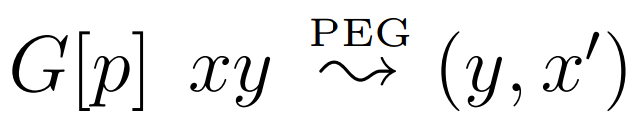
\includegraphics[width=0.3\textwidth]{pics/pegRel}
\end{center}                                      
\begin{itemize}
  \item Выражение \textit{p} парсит строку \textit{xy}, съедая \textit{x} и оставляя \textit{y}, возвращая 
\textit{x'} как результат
  \item Если справа \textit{fail}, значит, распарсить строку не удалось
\end{itemize}
\end{frame}

\begin{frame}[fragile]
  \transwipe[direction=90]
  \frametitle{Операционная семантика PEG: пустая строка}
\begin{center}
  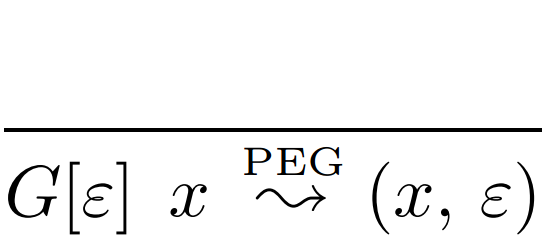
\includegraphics[width=0.3\textwidth]{pics/empty}
\end{center}                                      
\end{frame}

\begin{frame}[fragile]
  \transwipe[direction=90]
  \frametitle{Операционная семантика PEG: терминал}
\begin{center}
  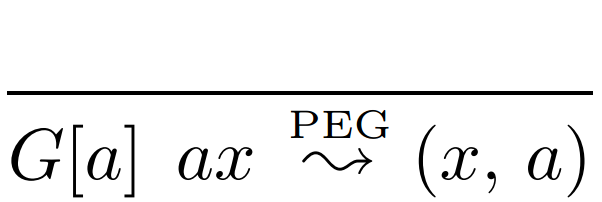
\includegraphics[width=0.35\textwidth]{pics/char1}  \\~\\   \pause
  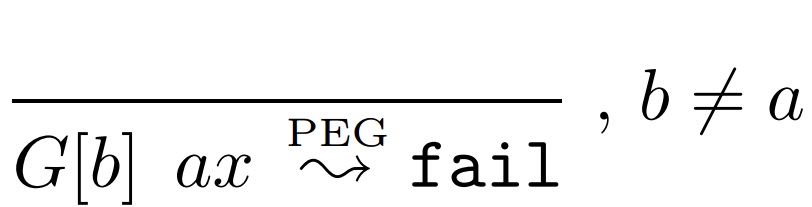
\includegraphics[width=0.5\textwidth]{pics/char2}   \\~\\   \pause
  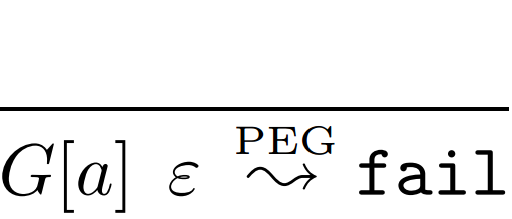
\includegraphics[width=0.3\textwidth]{pics/char3}
\end{center}  
\end{frame}

\begin{frame}[fragile]
  \transwipe[direction=90]
  \frametitle{Операционная семантика PEG: переменная}
\begin{center}
  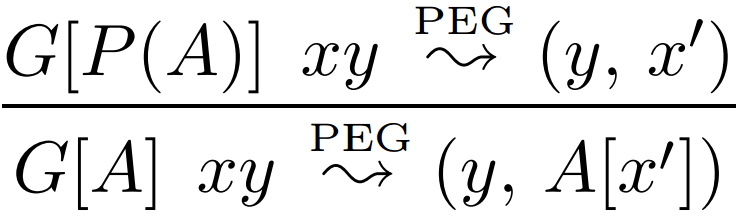
\includegraphics[width=0.4\textwidth]{pics/var1}  \\~\\     \pause
  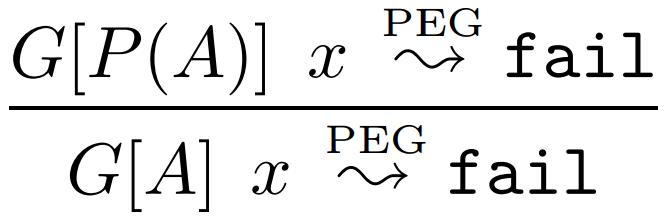
\includegraphics[width=0.35\textwidth]{pics/var2} 
\end{center}
\end{frame}


\begin{frame}[fragile]
  \transwipe[direction=90]
  \frametitle{Операционная семантика PEG: последовательность}
\begin{center}
  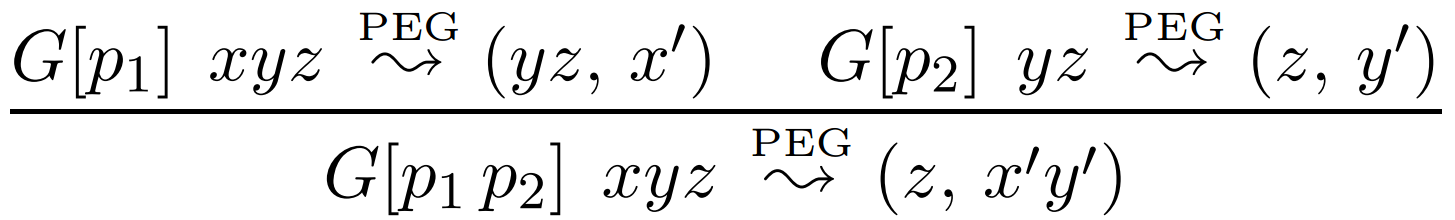
\includegraphics[width=0.7\textwidth]{pics/con1}  \\~\\     \pause
  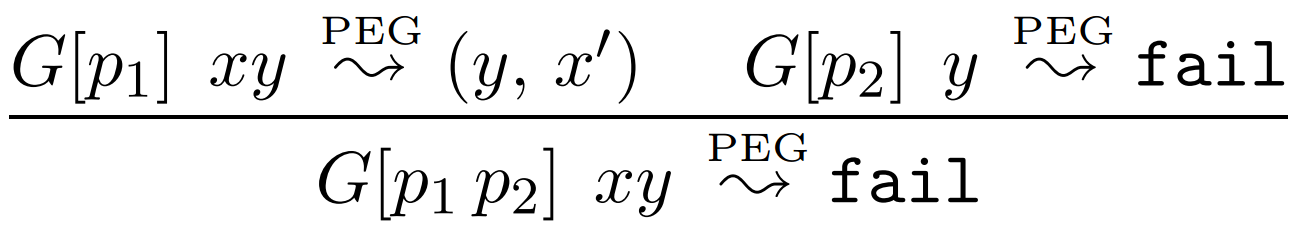
\includegraphics[width=0.7\textwidth]{pics/con2}  \\~\\     \pause
  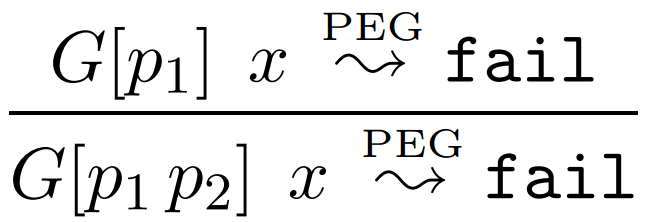
\includegraphics[width=0.35\textwidth]{pics/con3}
\end{center}
\end{frame}

\begin{frame}[fragile]
  \transwipe[direction=90]
  \frametitle{Операционная семантика PEG: выбор}
\begin{center}
  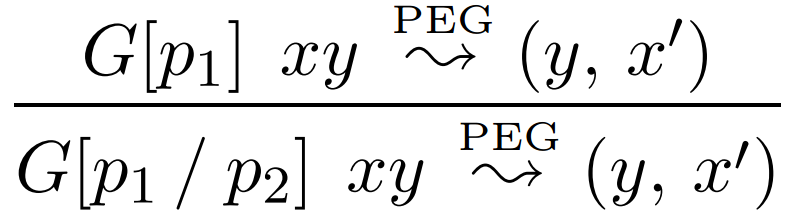
\includegraphics[width=0.4\textwidth]{pics/ord1}  \\~\\     \pause
  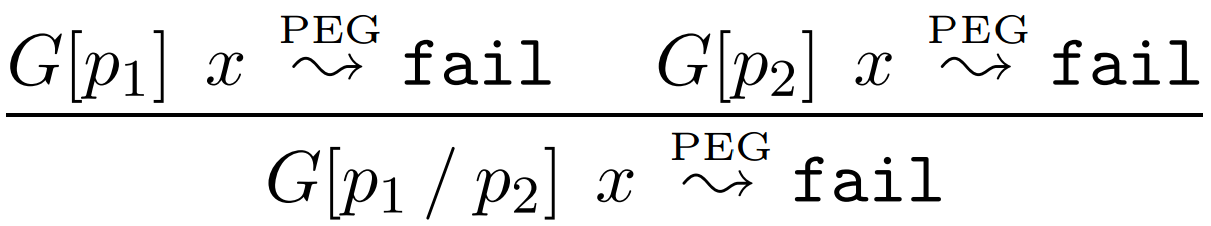
\includegraphics[width=0.6\textwidth]{pics/ord2}  \\~\\     \pause
  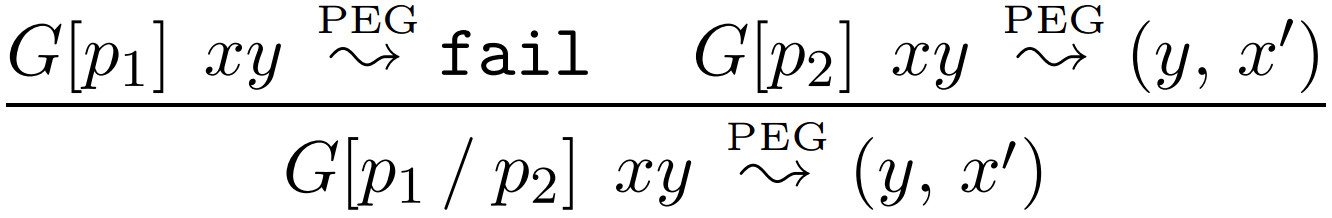
\includegraphics[width=0.65\textwidth]{pics/ord3}
\end{center}
\end{frame}

\begin{frame}[fragile]
  \transwipe[direction=90]
  \frametitle{Операционная семантика PEG: предикат не}
\begin{center}
  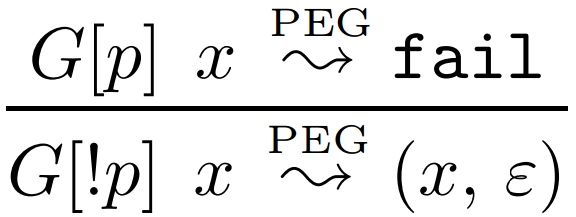
\includegraphics[width=0.3\textwidth]{pics/not1}  \\~\\     \pause
  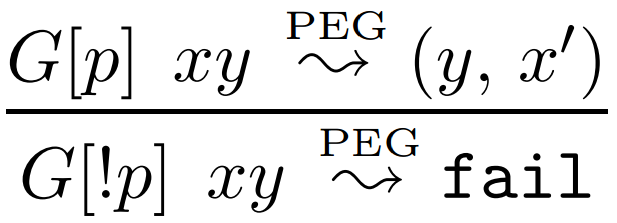
\includegraphics[width=0.35\textwidth]{pics/not2} 
\end{center}
\end{frame}

\begin{frame}[fragile]
  \transwipe[direction=90]
  \frametitle{Операционная семантика PEG: повторение}
\begin{center}
  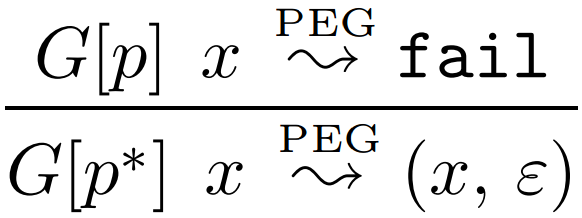
\includegraphics[width=0.3\textwidth]{pics/rep1}  \\~\\     \pause
  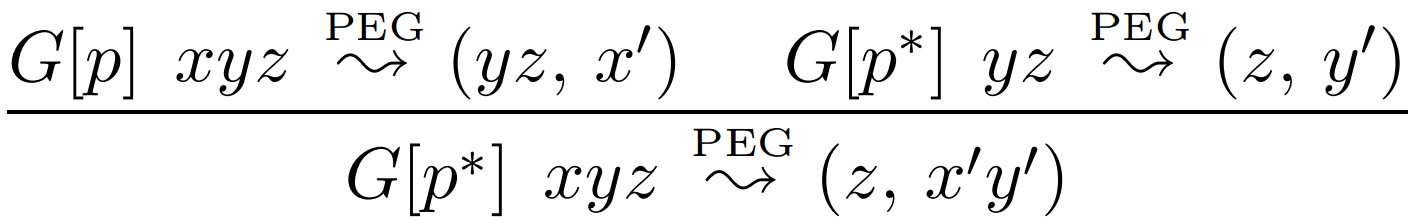
\includegraphics[width=0.7\textwidth]{pics/rep2} 
\end{center}
\end{frame}


\begin{frame}[fragile]
  \transwipe[direction=90]
  \frametitle{Преимущества и недостатки PEG}
  \begin{itemize}
    \item Преимущества
    \begin{itemize}
      \item Никаких неоднозначностей
      \item Наглядность
      \item Синтаксический анализатор и спецификация языка --- по сути одно и то же
      \item Синтаксический анализ за $O(n)$
    \end{itemize}
    \item Недостатки
    \begin{itemize}
      \item Жадность: разбирается наиболее большой префикс
      \begin{itemize}
        \item PEG $a^* a$ не может разобрать ничего
      \end{itemize}
      \item Никто не знает, какой именно класс языков можно распознать
      \begin{itemize}
        \item Все регулярные языки распознаются
        \item Все $LL(k)$ языки распознаются
        \item Не все КС языки распознаются
        \item Язык палиндромов $S \rightarrow x S x / x$ не распознается
        \item Язык $\{ a^n b^n c^n \, | \, n \geq 0 \}$ --- не КС --- распознается 
      \end{itemize}
	  \item Проблемы с левой рекурсией
    \end{itemize}
  \end{itemize}
\end{frame}

\begin{frame}[fragile]
  \transwipe[direction=90]
  \frametitle{Еще примеры: арифметические выражения}
  $$
  \begin{array}{crcl}
  &Expr  & \rightarrow & Sum \\
  &Sum & \rightarrow & Product \, ((+ \, / \, -) \, Product)^* \\
  &Product  & \rightarrow & Value \, ((* \, / \, /) \, Value)^* \\
  &Value & \rightarrow & [0-9] \, / \, ( \, Expr \, )
  \end{array}
  $$ 
\end{frame}

\begin{frame}[fragile]
  \transwipe[direction=90]
  \frametitle{Еще примеры: вложенные комментарии}
  $$
  \begin{array}{crcl}
  &Begin & \rightarrow & (* \\
  &End & \rightarrow & *) \\
  &C& \rightarrow & Begin \, N^* \, End \\
  &N& \rightarrow & C \, (!Begin \, !End \, Z)\\
  &Z& \rightarrow & any \, single \, character
  \end{array}
  $$ 
\end{frame}

\begin{frame}[fragile]
  \transwipe[direction=90]
  \frametitle{Еще примеры: не КС язык}
  $$
  \begin{array}{crcl}
  &S & \rightarrow & \& (A \, c) \, a^+ \, B \, !. \\
  &A & \rightarrow & a \, A? \, b \\
  &B & \rightarrow & b \, B? \, c \\
  \end{array}
  $$ 
\end{frame}

\begin{frame}[fragile]
  \transwipe[direction=90]
  \frametitle{Борьба с левой рекурсией: ограниченная левая рекурсия}
\begin{itemize}
  \item $A^n$ имеет не более $n$ леворекурсивных вызовов $A$, $A^0$ всегда 
завершается ошибкой
\end{itemize}
$$
\begin{array}{crcl}
&E^0 & ::= & fail \\ 
&E^1 & ::= & E^0 + n / n = \bot + n / n = n \\
&E^2 & ::= & E^1 + n / n = n + n / n \\
&E^3 & ::= & E^2 + n / n = (n + n / n) + n / n\\
& & \dots &  \\
&E^n & ::= & E^{n-1} + n / n \\
\end{array}
$$ 
\end{frame}

\begin{frame}[fragile]
  \transwipe[direction=90]
  \frametitle{Борьба с левой рекурсией}
\begin{itemize}
  \item Ищем значение $n$ для каждого леворекурсивного нетерминала
  \item Подбирается такая граница, чтобы префикс, обработанный правилом, имел 
максимальную длину
  \item Промежуточные значения сохраняются в табличку $L$
  \begin{itemize}
    \item $L[(A, x) \rightarrow X](B, y) = L(B, y)$, если $B \neq A$ или $y 
\neq x$
    \item $L[(A, x) \rightarrow X](A, x) = X$
  \end{itemize}
\end{itemize}
\end{frame}

\begin{frame}[fragile]
  \transwipe[direction=90]
  \frametitle{Обработка леворекурсивного нетерминала}
\begin{center}
  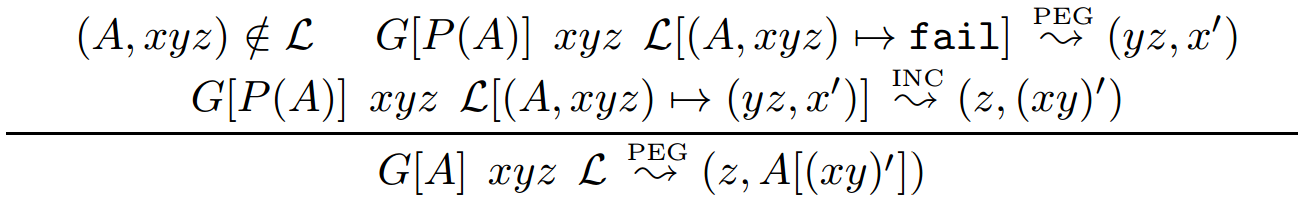
\includegraphics[width=1.0\textwidth]{pics/lvar1}  \\~\\     \pause
  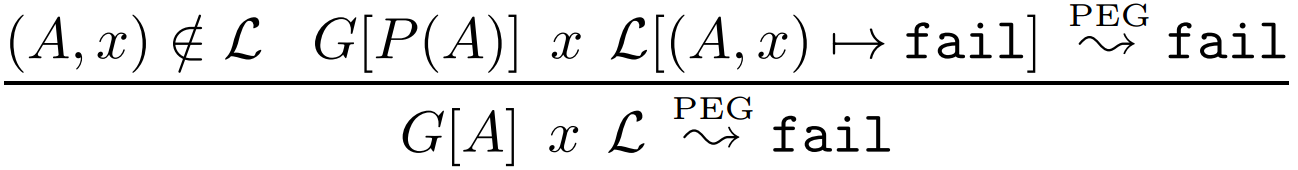
\includegraphics[width=0.7\textwidth]{pics/lvar2}  \\~\\     \pause 
  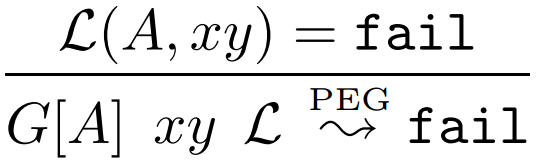
\includegraphics[width=0.3\textwidth]{pics/lvar3}  \\~\\     \pause
  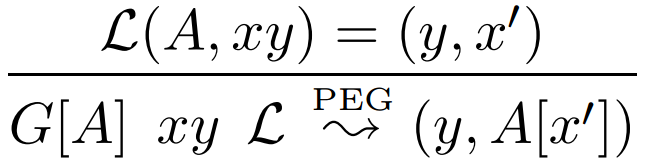
\includegraphics[width=0.35\textwidth]{pics/lvar4}  
\end{center}
\end{frame}

\begin{frame}[fragile]
  \transwipe[direction=90]
  \frametitle{Семантика отношения INC}
\begin{center}
  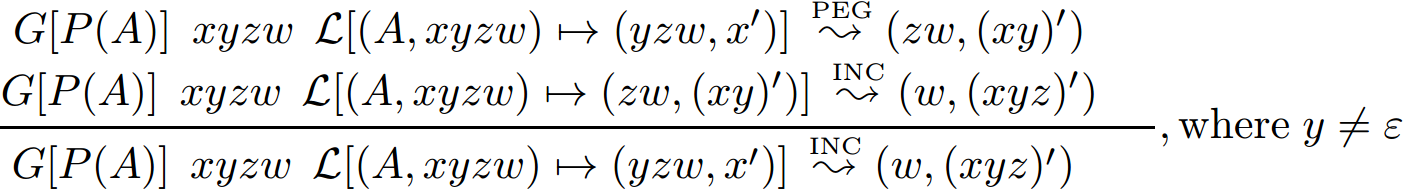
\includegraphics[width=1.0\textwidth]{pics/incr1}  \\~\\     \pause
  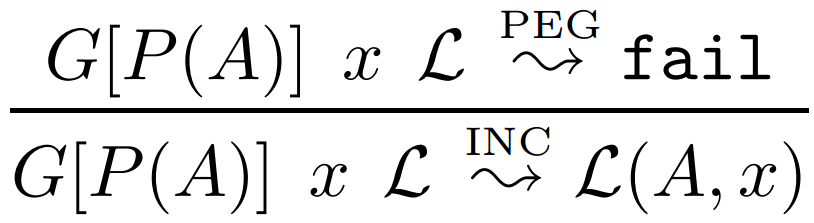
\includegraphics[width=0.3\textwidth]{pics/incr2}  \\~\\     \pause
  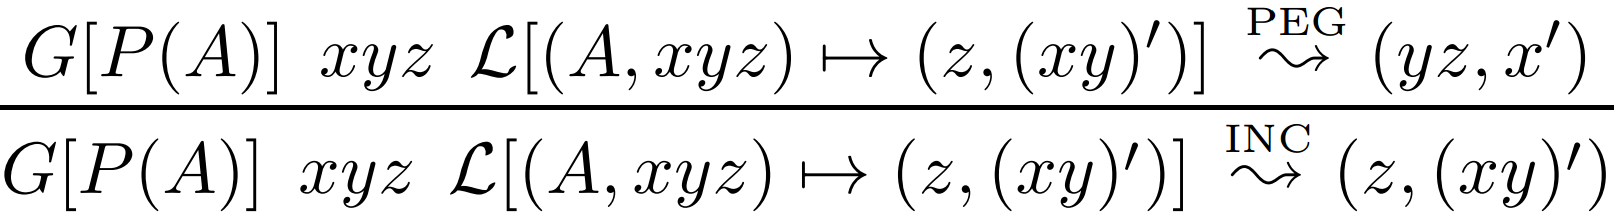
\includegraphics[width=0.7\textwidth]{pics/incr3}  
\end{center}
\end{frame}

\end{document}
